\documentclass[a4paper, 12pt, slovene]{article}
\usepackage[slovene]{babel}
\usepackage[utf8]{inputenc}
\usepackage{lmodern}
\usepackage[T1]{fontenc}
\usepackage{graphicx}
\usepackage{caption}
\captionsetup{font=footnotesize}
\usepackage{fullpage}
\usepackage{enumitem}
\usepackage{array}
\usepackage{wrapfig}
\usepackage{multirow}
\usepackage{tabularx}
\usepackage{amsmath}
\usepackage{amssymb}
\usepackage{subcaption}
\newcommand*\diff{\mathop{}\!\mathrm{d}}
\newcommand*\Diff[1]{\mathop{}\!\mathrm{d^#1}}
\newcommand*\difft{\mathop{}\!\ddot{ }}
\usepackage{float}
\usepackage{mathrsfs}
\usepackage{fancyvrb}
\usepackage{hyperref}
\usepackage{xurl}
\usepackage{breqn}
\numberwithin{equation}{section}

\newcommand{\Ai}{\mathrm{Ai}}
\newcommand{\Bi}{\mathrm{Bi}}

\renewcommand{\Re}{\mathop{\rm Re}\nolimits}
\renewcommand{\Im}{\mathop{\rm Im}\nolimits}
\newcommand{\Tr}{\mathop{\rm Tr}\nolimits}
\newcommand{\diag}{\mathop{\rm diag}\nolimits}
\newcommand{\dd}{\,\mathrm{d}}
\newcommand{\ddd}{\mathrm{d}}
\newcommand{\ii}{\mathrm{i}}
\newcommand{\lag}{\mathcal{L}\!}
\newcommand{\ham}{\mathcal{H}\!}
\newcommand{\four}[1]{\mathcal{F}\!\left(#1\right)}
\newcommand{\bigO}[1]{\mathcal{O}\!\left(#1\right)}
\newcommand{\sh}{\mathop{\rm sinh}\nolimits}
\newcommand{\ch}{\mathop{\rm cosh}\nolimits}
\renewcommand{\th}{\mathop{\rm tanh}\nolimits}
\newcommand{\erf}{\mathop{\rm erf}\nolimits}
\newcommand{\erfc}{\mathop{\rm erfc}\nolimits}
\newcommand{\sinc}{\mathop{\rm sinc}\nolimits}
\newcommand{\rect}{\mathop{\rm rect}\nolimits}
\newcommand{\ee}[1]{\cdot 10^{#1}}
\newcommand{\inv}[1]{\left(#1\right)^{-1}}
\newcommand{\invf}[1]{\frac{1}{#1}}
\newcommand{\sqr}[1]{\left(#1\right)^2}
\newcommand{\half}{\frac{1}{2}}
\newcommand{\thalf}{\tfrac{1}{2}}
\newcommand{\pd}{\partial}
\newcommand{\Dd}[3][{}]{\frac{\ddd^{#1} #2}{\ddd #3^{#1}}}
\newcommand{\Pd}[3][{}]{\frac{\pd^{#1} #2}{\pd #3^{#1}}}
\newcommand{\avg}[1]{\left\langle#1\right\rangle} 
\newcommand{\norm}[1]{\left\Vert #1 \right\Vert}
\newcommand{\braket}[2]{\left\langle #1 \vert#2 \right\rangle}
\newcommand{\obraket}[3]{\left\langle #1 \vert #2 \vert #3 \right \rangle}
\newcommand{\hex}[1]{\texttt{0x#1}}

\renewcommand{\iint}{\mathop{\int\mkern-13mu\int}}
\renewcommand{\iiint}{\mathop{\int\mkern-13mu\int\mkern-13mu\int}}
\newcommand{\oiint}{\mathop{{\int\mkern-15mu\int}\mkern-21mu\raisebox{0.3ex}{$\bigcirc$}}}

\newcommand{\wunderbrace}[2]{\vphantom{#1}\smash{\underbrace{#1}_{#2}}}

\renewcommand{\vec}[1]{\overset{\smash{\hbox{\raise -0.42ex\hbox{$\scriptscriptstyle\rightharpoonup$}}}}{#1}}
\newcommand{\bec}[1]{\mathbf{#1}}

\newcommand{\bi}[1]{\hbox{\boldmath{$#1$}}}
\newcommand{\bm}[1]{\hbox{\underline{$#1$}}}  

\newcommand{\nap}{\nabla_{\perp}}  

\catcode`_=12
\begingroup\lccode`~=`_\lowercase{\endgroup\let~\sb}
\mathcode`_="8000


\begin{document}

\begin{titlepage}
\title{\textsc{Model vožnje skozi semafor: variacijska metoda} \\[1ex] \large Prva naloga pri predmetu Modelska analiza 1}
\author{Gašper Lotrič \\ 28191019}
\date{oktober 2022}

\maketitle
\end{titlepage}

\tableofcontents
\pagebreak


\section{Naloga}
Varčno vožnjo lahko defniramo s pogojem, da je pospeševanja in zaviranja čim manj. To lahko dosežemo z minimizacijo kumulativnega kvadrata pospeška. Iščemo optimalni režim vožnje v situaciji, ko poskušamo razdaljo do semaforja prevoziti ravno v trenutku, ko se prižge zelena luč.


\section{Formulacija problema}
Avto se vozi s trenutno hitrostjo $v_0$, ko se pred njim na razdalji $l$ pojavi semafor s prižgano rdečo lučjo. Do semaforja mora pripeljati v času $t_0$, ko se bo prižgala zelena luč. Kriterija za optimalno vožnjo sta čim večja hitrost pri semaforju in čim manj pospeševanja ali zaviranja.


Do semaforja moramo priti natanko tedaj, ko se prižge zelena luč (ali kasneje), torej mora veljati
\begin{equation}
\int_0^{t_0}v(t)\diff t = l
\label{e:vez}
\end{equation}
Za pogoj za čim bolj udobno vožnjo izberemo minimizacijo kumulativnega kvadrata pospeška
\begin{equation}
\int_0^{t_0}\dot{v}^2(t)\diff t = \rm{min.}
\end{equation}
Varčno vožnjo definiramo s funkcionalom, kjer $\lag$ predstavlja Lagrangevo funkcijo.
\begin{equation}
F(v) = \int_0^{t_0}\lag(v, \dot{v}, t)\diff t
\end{equation}
optimalno vožnjo dosežemo, ko minimiziramo $F(v)$. V tem primeru minimiziramo kvadrat pospeška in smo omejeni z vezjo \eqref{e:vez} tako, da je
\begin{equation}
\lag = \dot{v}^2 - \lambda v.
\end{equation}


\subsection{Brezdimenzijska oblika}
Problem prepišemo v brezdimenzijsko obliko. Hitrost normiramo z začetno, čas s časom $t_0$ in razdaljo $l$ s produktom $v_0t_0$.
\begin{eqnarray}
t	&\rightarrow &	x = t/t_0	\\
v	&\rightarrow &	y = v/v_0	\\
l	&\rightarrow & z = l/v_0t_0
\end{eqnarray}
začetni pogoj $v(0) = v_0$ se prepiše v $y(0) = 1$, pogoj da prevozimo semafor ravno ob času $t = t_0$ pa v
\begin{equation}
\int_0^1y(x)\diff x = z
\label{e:vez2}
\end{equation}
Lagrangian pa se prevede v $\lag' = \dot{y}^2 - \lambda y$. Tako dobimo funkcional $F'$, ki ga minimiziramo.
\begin{equation}
F'(y) = \int_0^1\lag'(y, \dot{y}, x)\diff x
\end{equation}


\subsection{Euler-Lagrangeove enačbe}
V brezdimenzijskem sistemu zapišemo Euler-Lagrangevi enačbo kot
\begin{eqnarray}
\frac{\diff}{\diff x}\Pd{\lag'}{\dot{y}} - \Pd{\lag'}{y} &=& 0 \\
\Dd{}{t}2\dot{y} + \lambda &=& 0.
\end{eqnarray}
Sledi, da je $\ddot{y} = - \frac{\lambda}{2}$. To dvakrat integriramo in dobimo splošno obliko funkcije hitrosti za ta primer
\begin{equation}
y(t) = -\frac{\lambda}{4}x^2 + Ax + B.
\label{e:hitrost-spl}
\end{equation}
Iz začetnega pogoja $y(x=0) = 1$ dobimo parameter $B=1$. Upotševamo tudi to, da si želimo semafor prevoziti pri ekstremalni hitrosti $\dot{y}(x=1) = 0$ in iz tega pogoja bomo dobili še parameter $A=\lambda/2$. Funkcijo hitrosti \eqref{e:hitrost-spl} zdaj lahko zapišemo z znanimi parametri.
\begin{equation}
y(x) = -\frac{\lambda}{4}x^2 + \frac{\lambda}{2}x + 1
\label{e:hitrost-mid}
\end{equation}
Lagrangeev multiplikator $\lambda$ pa izračunamo s pomočjo pogoja \eqref{e:vez2}. Dobimo
\begin{equation}
\lambda = 6(z-1)
\end{equation}
in enačbo \eqref{e:hitrost-mid} prepišemo v končno obliko
\begin{equation}
y(x) = 3\left( z-1 \right)\left( x - \frac{x^2}{2}\right) + 1
\label{e:hitrost-fin}
\end{equation}
Za različne začetne hitrosti, ki se odražajo v parametru $z=l/t_0v_0$, dobimo potek brezdimenzijske hitrosti, ki je prikazan na sliki \ref{f:hitrosti-basic}.

\begin{figure}[H]
\centering
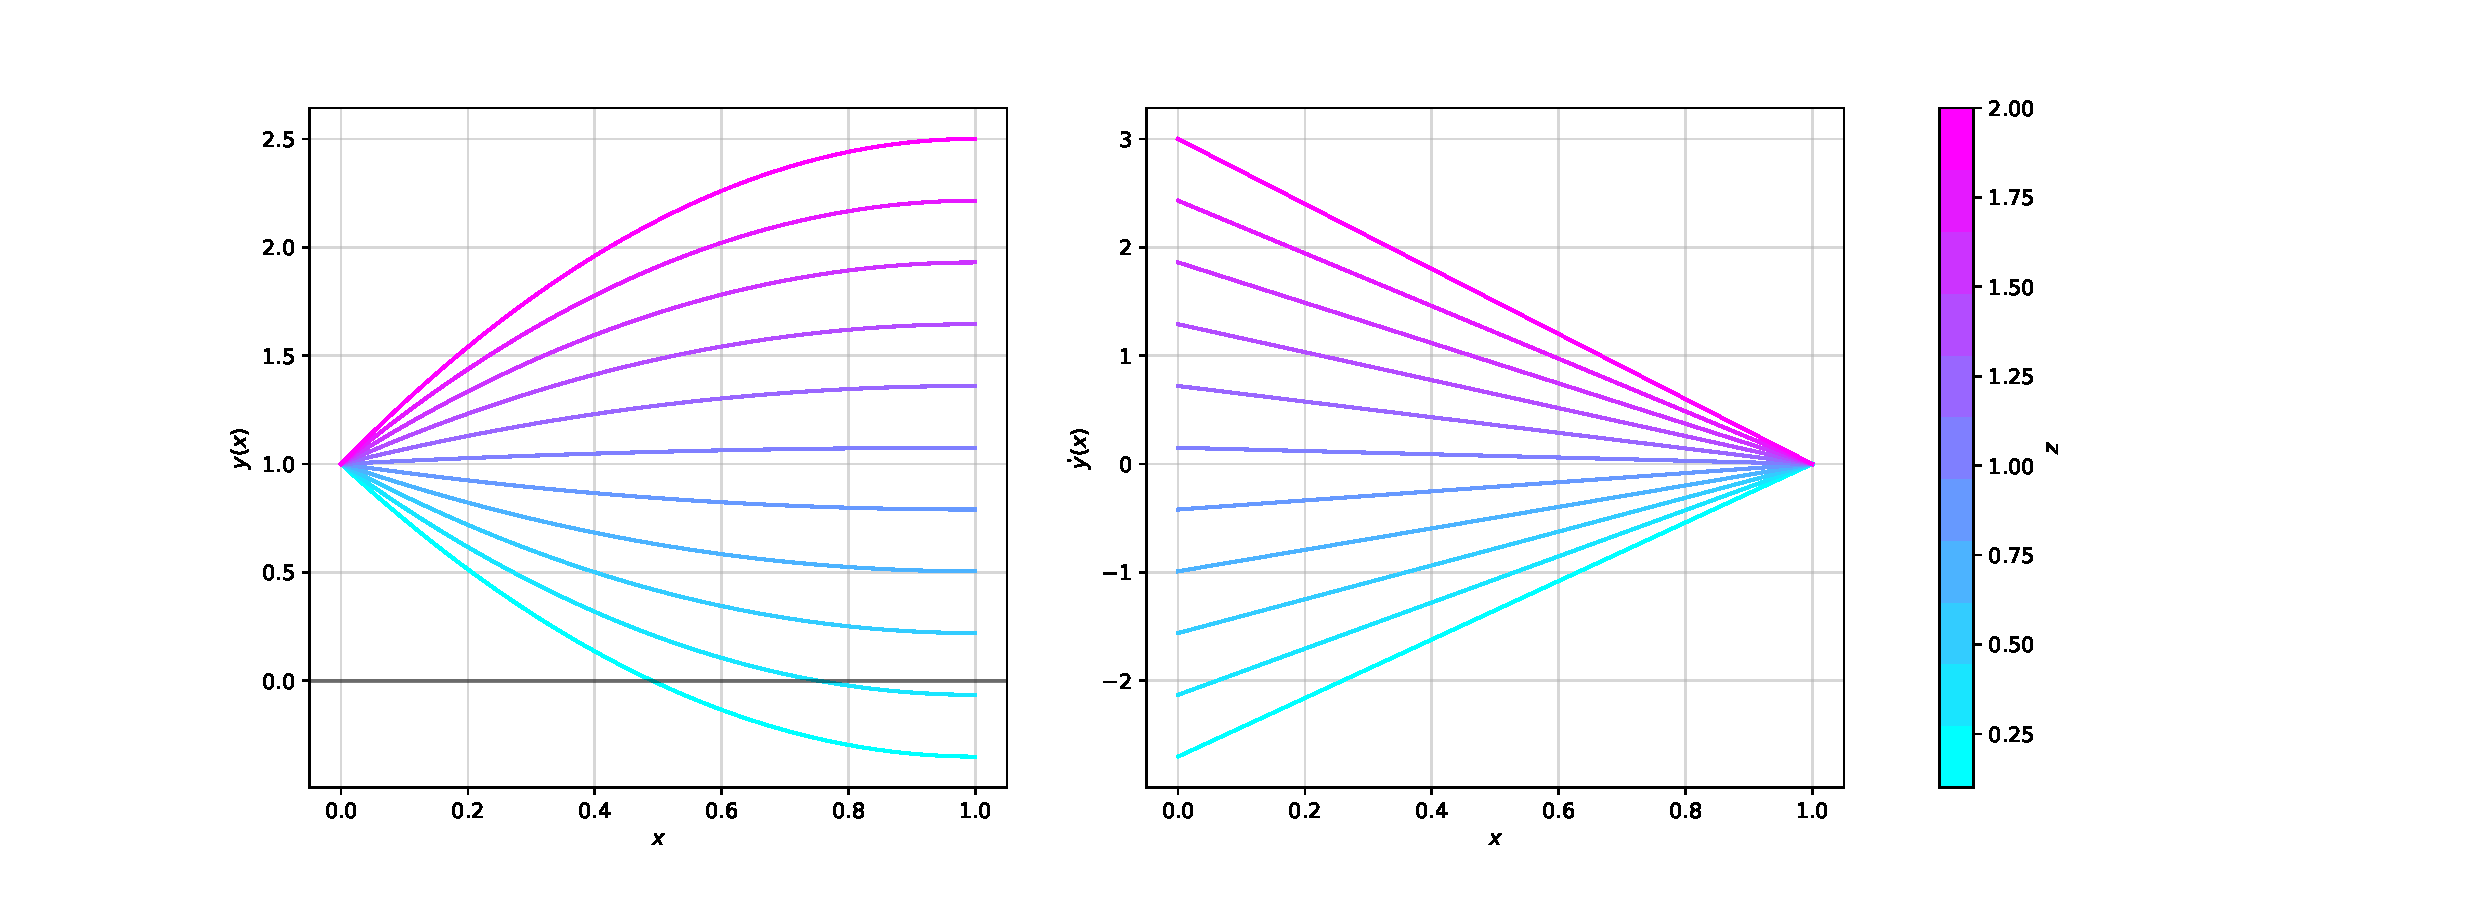
\includegraphics[width=0.95\textwidth]{grafi/hitrosti_basic.pdf}
\caption{Brezdimenzijska hitrost $y(x)$ za različne začetne hitrosti $v_0$, ki se odražajo v parametru $z$ na levi. Pospešek$\dot{y}(x)$ na desni.}
\label{f:hitrosti-basic}
\end{figure}

Vse krivulje se začnejo v $y=1$, ker so vsaka posebaj normirane s svojo začetno hitrostjo. Opazimo, da nas želja po udobni vožnji pripelje do nekaj nesmiselnih rešitev (spodnji dve krivulji levega grafa na sliki \ref{f:hitrosti-basic}), kjer dobimo negativno hitrost. To pomeni, da se peljemo mimo semaforja in potem vzvratno do črte, ki smo jo že prečkali.

\begin{eqnarray}
y(x) = 3\left( z-1 \right)\left( x - \frac{x^2}{2}\right) + 1 &\geq& 0	\\
z &\geq& 1-\frac{1}{3\left( x- \frac{x^2}{2}\right)}
\end{eqnarray}
Upoštevamo, da so funkcije hitrosti parabole s temenom v točki $x=1$, torej so na intervalu $x\in[0,1]$ monotone in dosežejo maksimum na koncu tega intervala. Zato je pogoj za pozitivno hitrost $z \geq 1/3$, torej $v_0 \leq 3l/t_0$. \par\vspace{5mm}

Bolj predstavljivo sliko dobimo, če pogledamo kaj se dogaja v sistemu z originalnimi koordinatami. V tem sistemu je rešitev enaka
\begin{equation}
v(t) = v_0 + \frac{3(l-v_0t_0)}{2t_0^3}\left( 2t_0t-t^2\right).
\end{equation}

\begin{figure}[H]
\centering
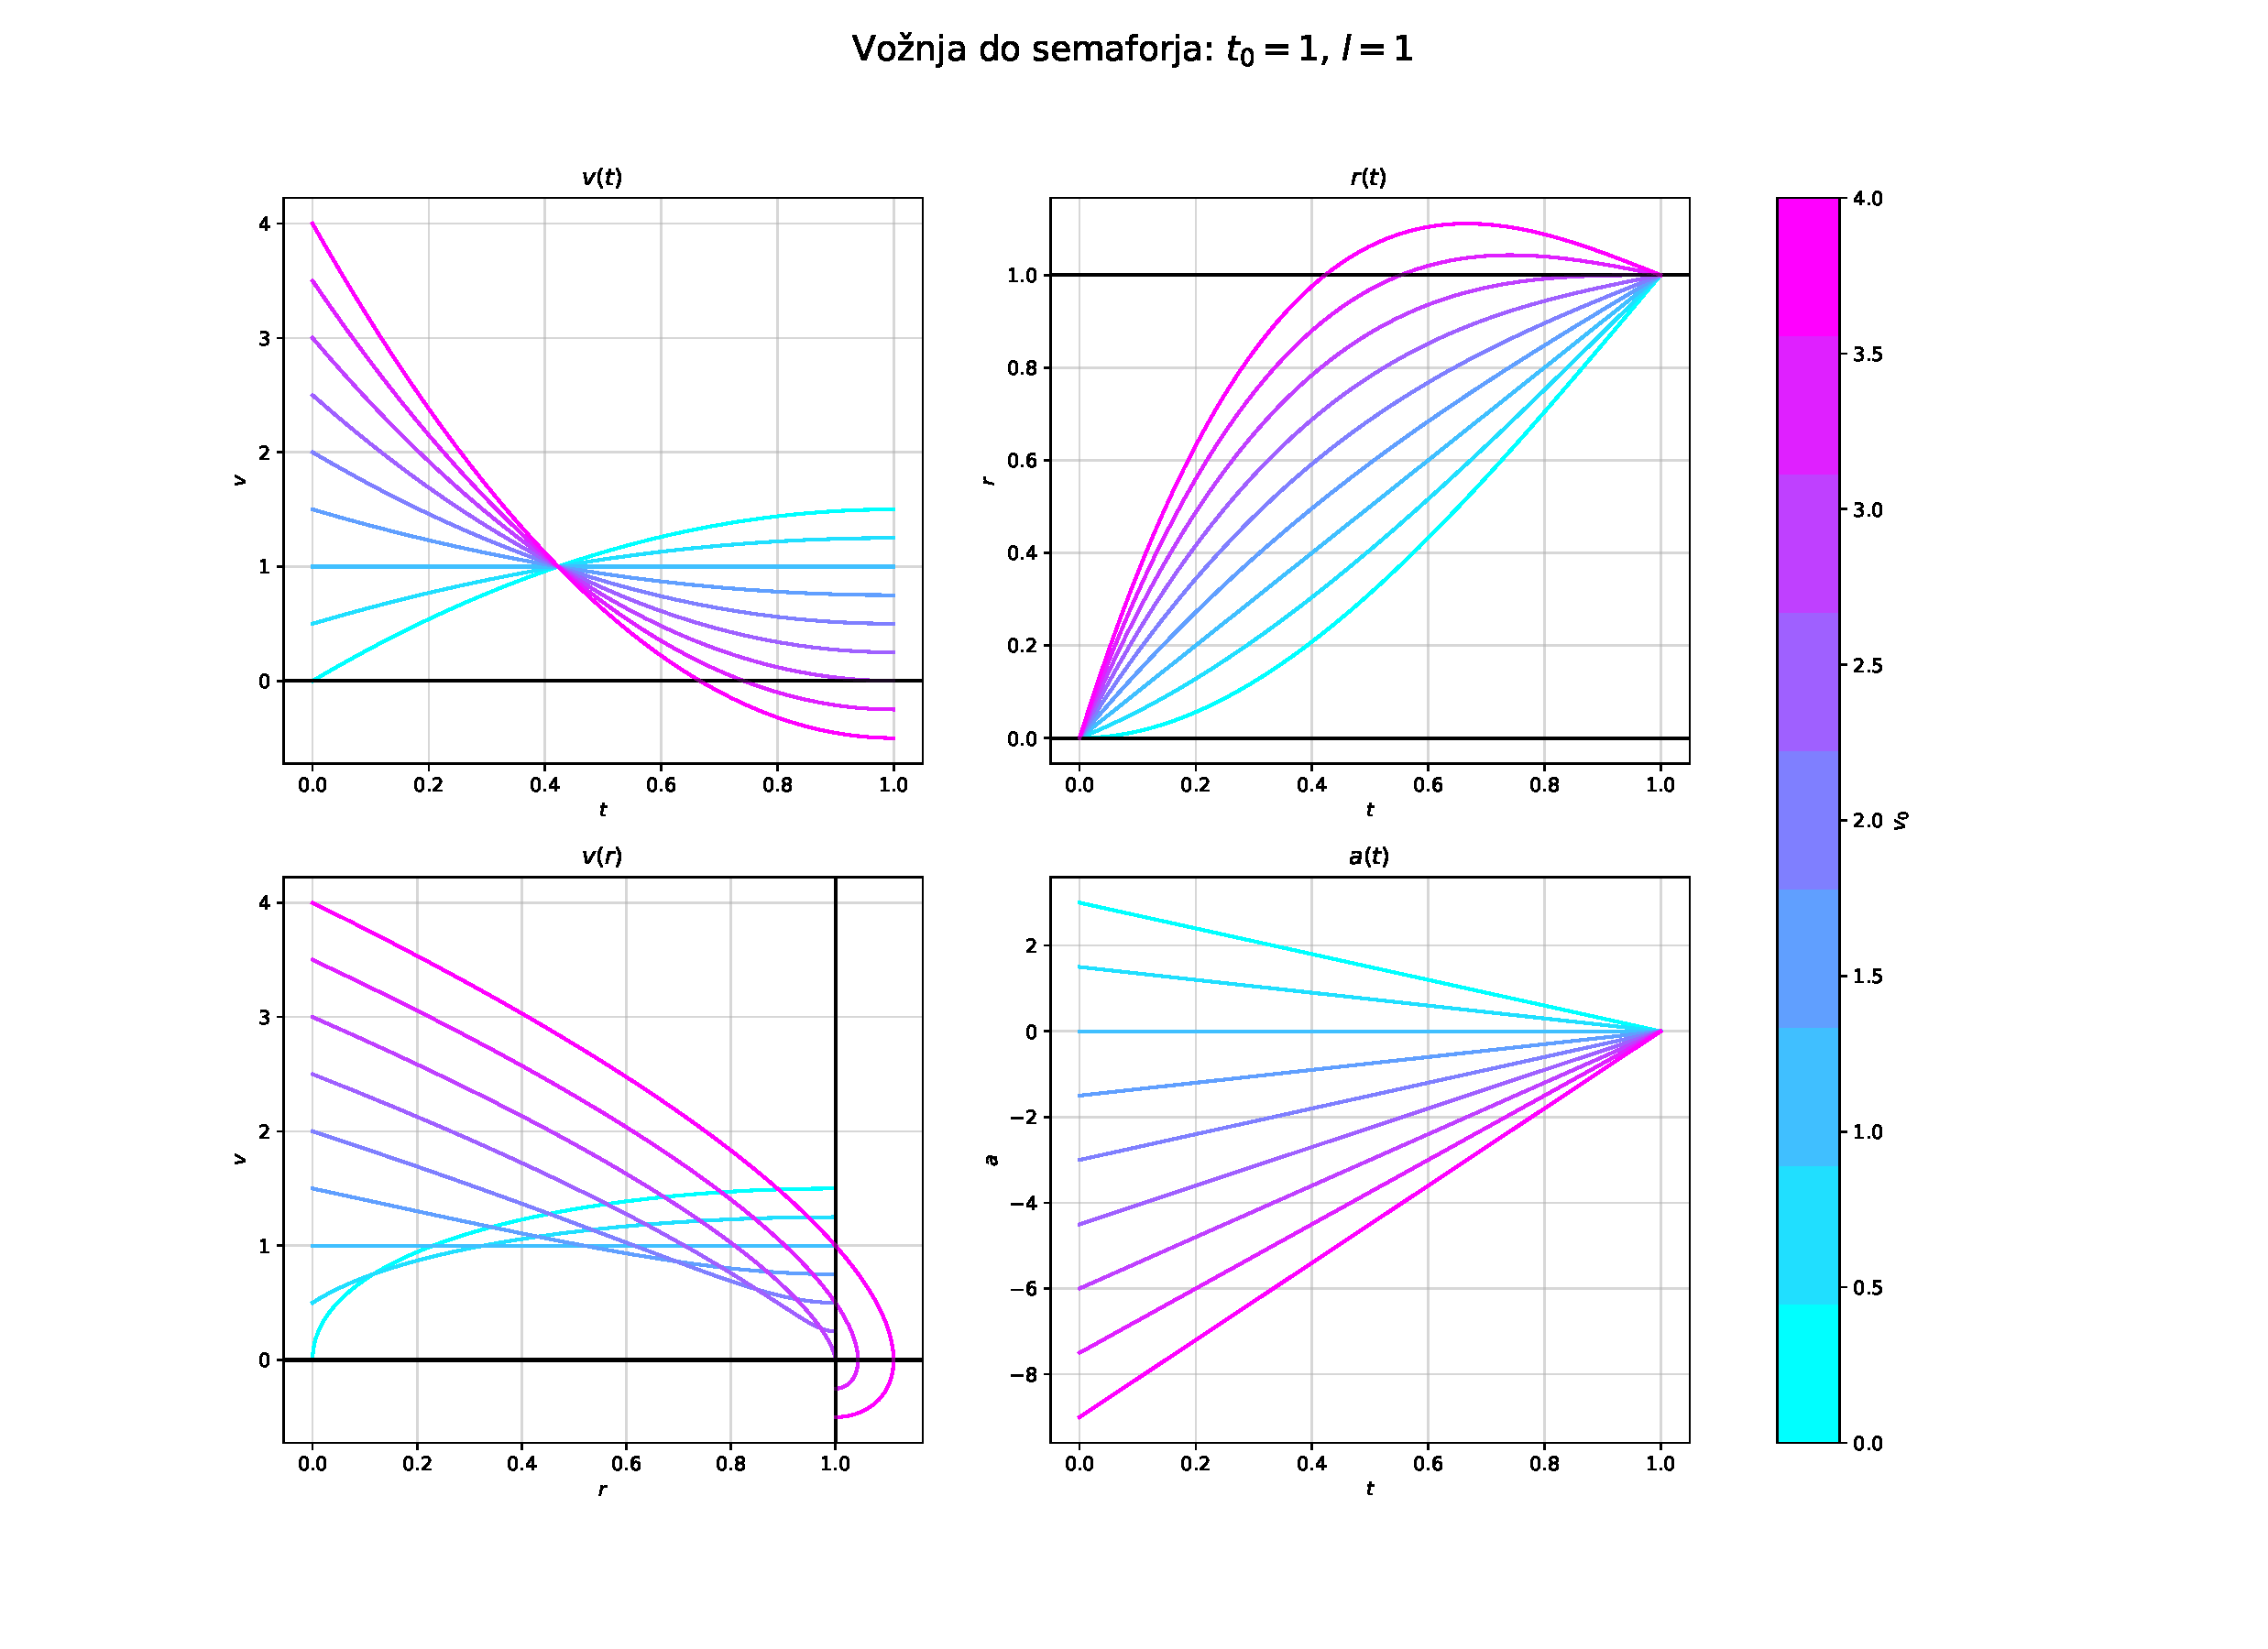
\includegraphics[width=0.95\textwidth]{grafi/dimenzijsko.pdf}
\caption{Hitrost v odvisnosti od časa, hitrost v odvisnosti od poti, pot v odvisnosti od časa in časovna odvisnost pospeška za semafor s parametri $t_0=1$, $l=1$.}
\label{f:hitrosti-4graf}
\end{figure}

Na sliki \ref{f:hitrosti-4graf} je nasrisana rešitev v koordinatah $v$ in $t$. Na levi strani hitrost v odvisnosti od časa in položaja, na desni pa časovna odvisnost poti in pospeška. Spet opazimo nesmiselnost nekaterih rešitev (negativna hitrost), kar je še bolj očitno na grafu poti (desno zgoraj). Še ena zanimivost se pojavi na grafu $v(t)$, kjer se vse krivulje sekajo v isti točki, torej ne glede na to s kakšno hitrostjo začnemo, se bomo ob nekem času peljali vedno z isto hitrostjo. To se zgodi v točki, kjer je $\pd v/\pd v_0=0$, torej ob času $t_1 = t_0 (1-\sqrt{3}/3)$.




\section{Radar tik za križiščem}
Tik za križiščem je postavljen radar z omejitvijo $\tilde{v}$. Vožnjo moramo prilagoditi tako, da ne dobimo kazni in ohranimo udobje vožnje. Torej rešujemo isti problem, le robni pogoj se spremeni v $v(t_0) = \tilde{v}$. Kot v prejšnjem poglavju, izpeljemo enačbo za hitrost
\begin{equation}
v(t) = \frac{3}{t_0^2}(2l-v_0t_0-\tilde{v}t_0)(t_0t-t^2) + \frac{\tilde{v}-v_0}{t_0}t + v_0.
\end{equation}

\begin{figure}[H]
\centering
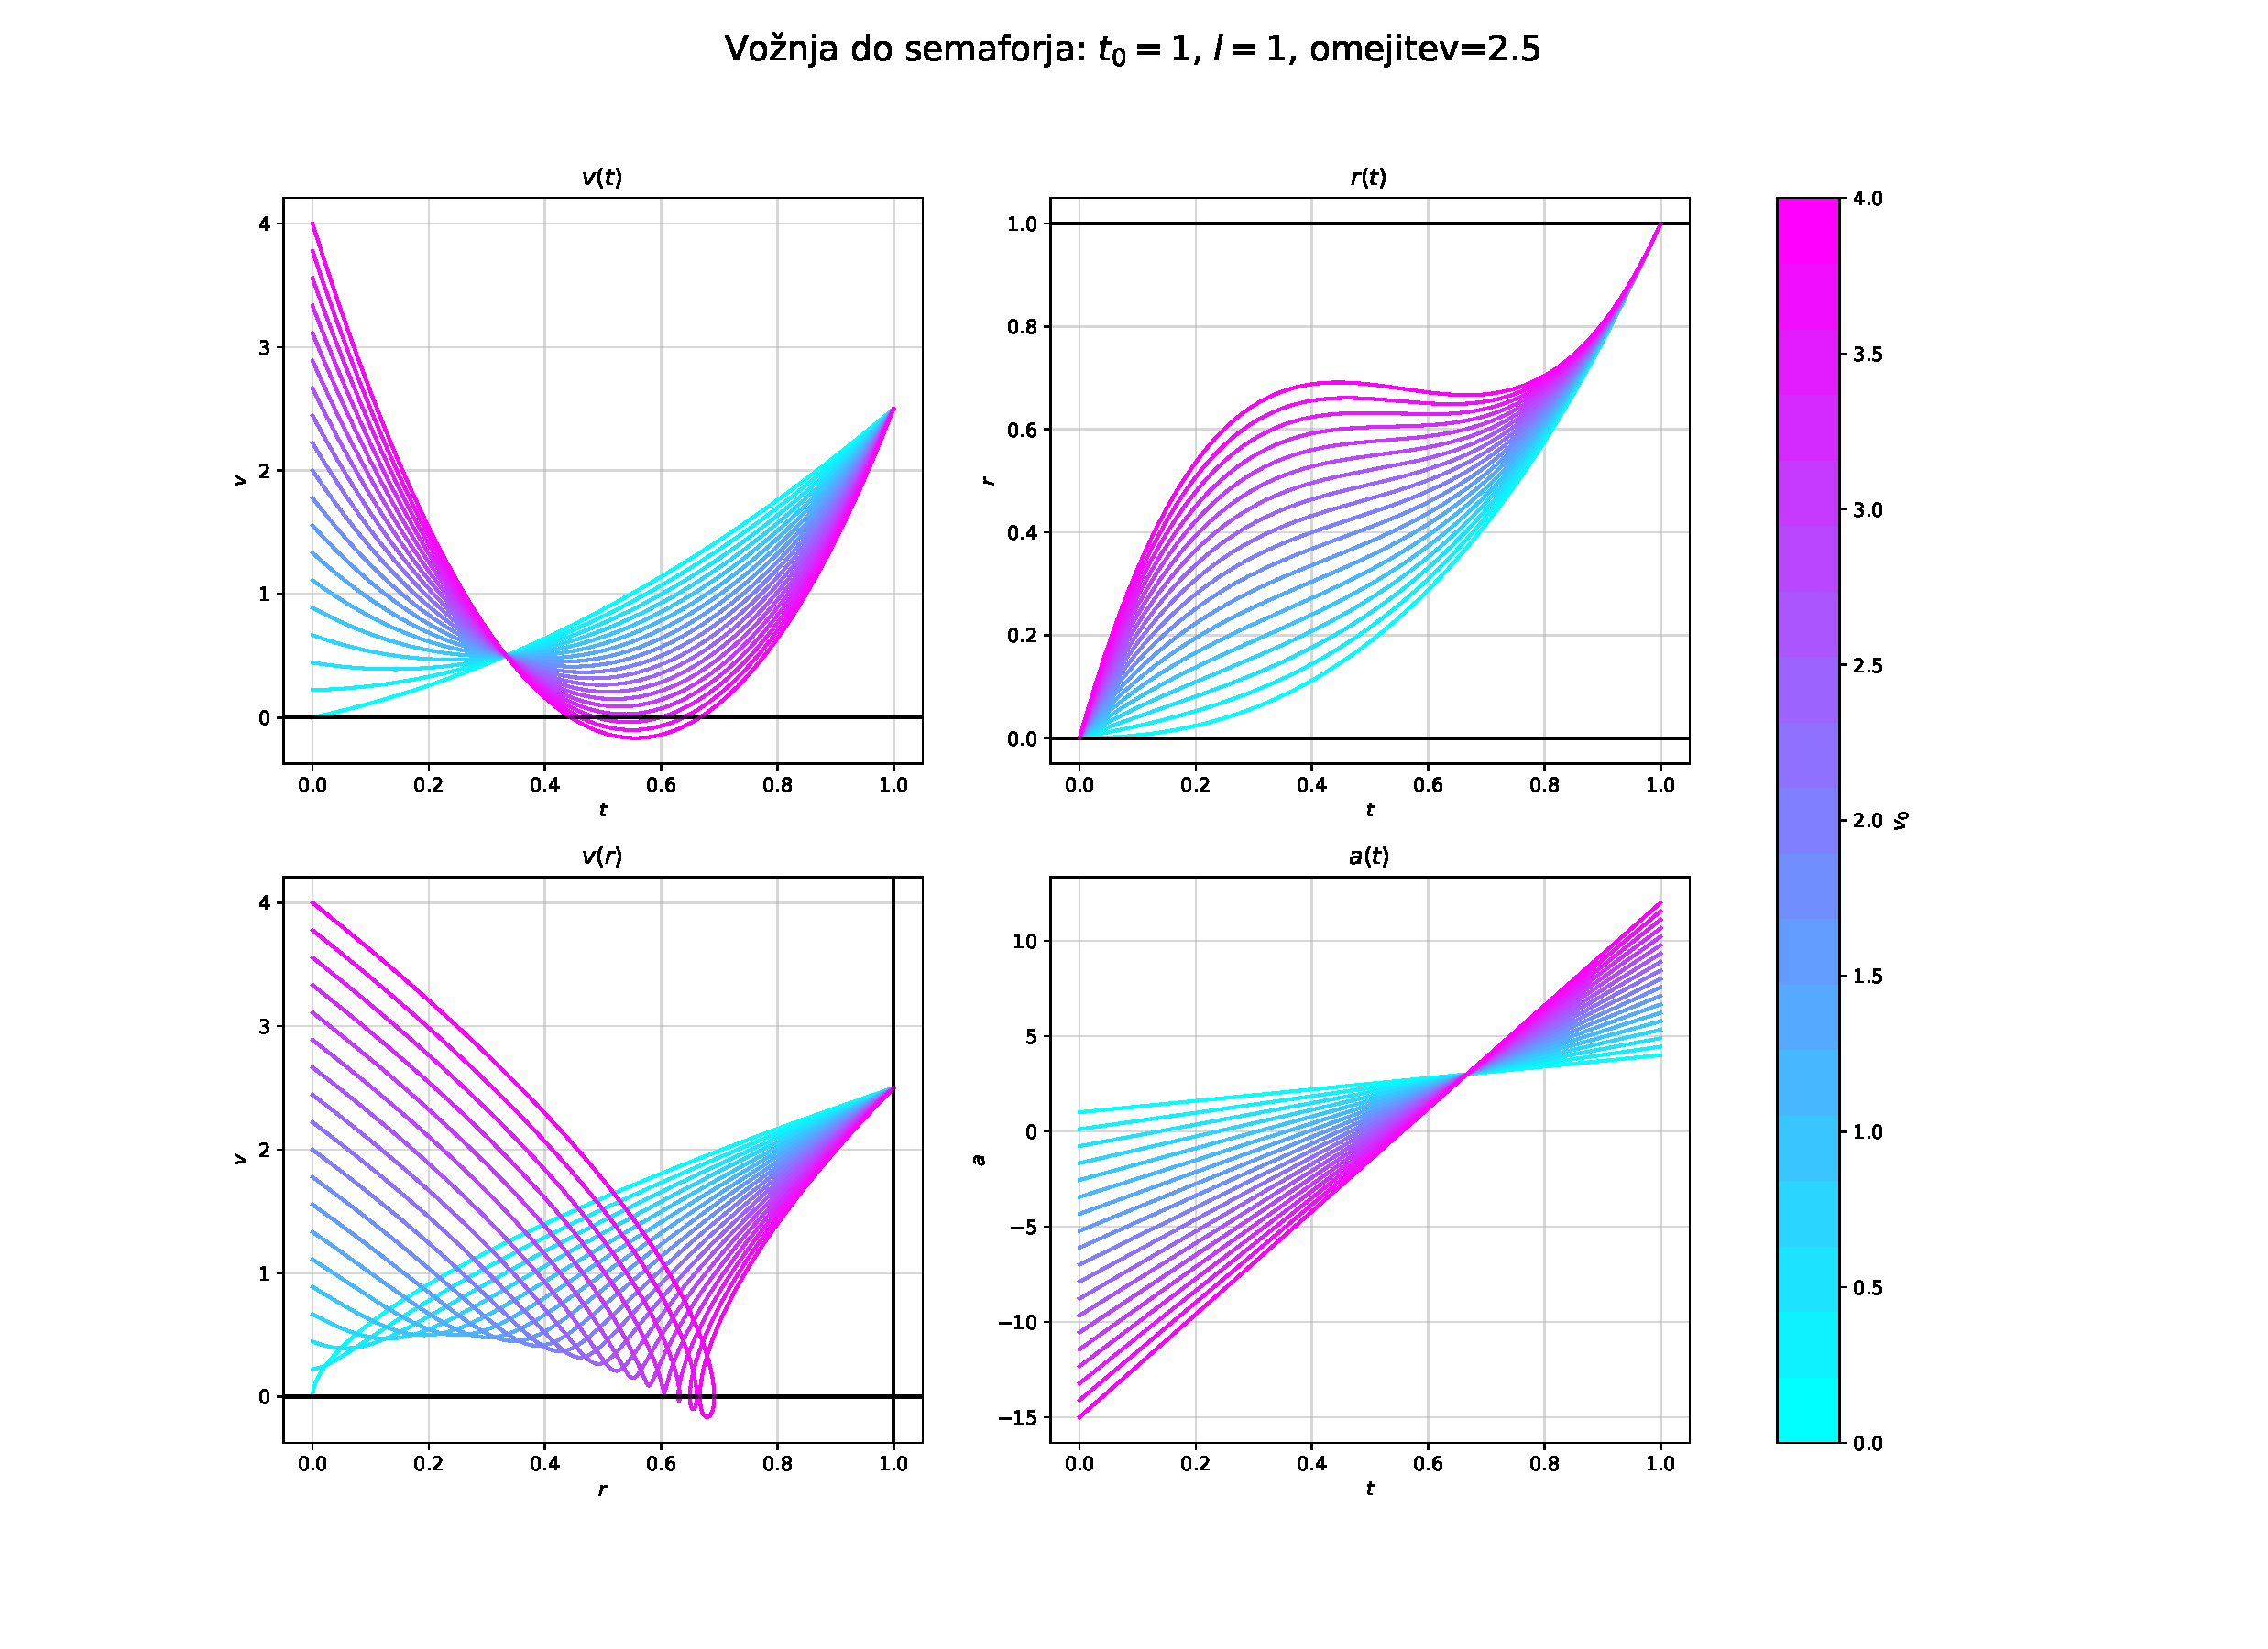
\includegraphics[width=0.95\textwidth]{grafi/dim_radar_1_1_2.5.pdf}
\caption{Hitrost v odvisnosti od časa, hitrost v odvisnosti od poti, pot v odvisnosti od časa in časovna odvisnost pospeška za semafor z radarjem s parametri $t_0=1$, $l=1$, $\tilde{v}=2.5$.}
\label{f:radar-4graf}
\end{figure}

Na sliki \ref{f:radar-4graf} vidimo, da se hitrost še vedno obnaša parabolično, le da ekstrm ni več na koncu poti ampak nekje vmes. Spet se vse hitrosti sekajo v isti točki, tokrat v $t_2 = 1/3$. Na sliki \ref{f:radar-omejitve} pa vidimo, kako na hitrosti vpliva omejitev $\tilde{v}$.

\begin{figure}[H]
\centering
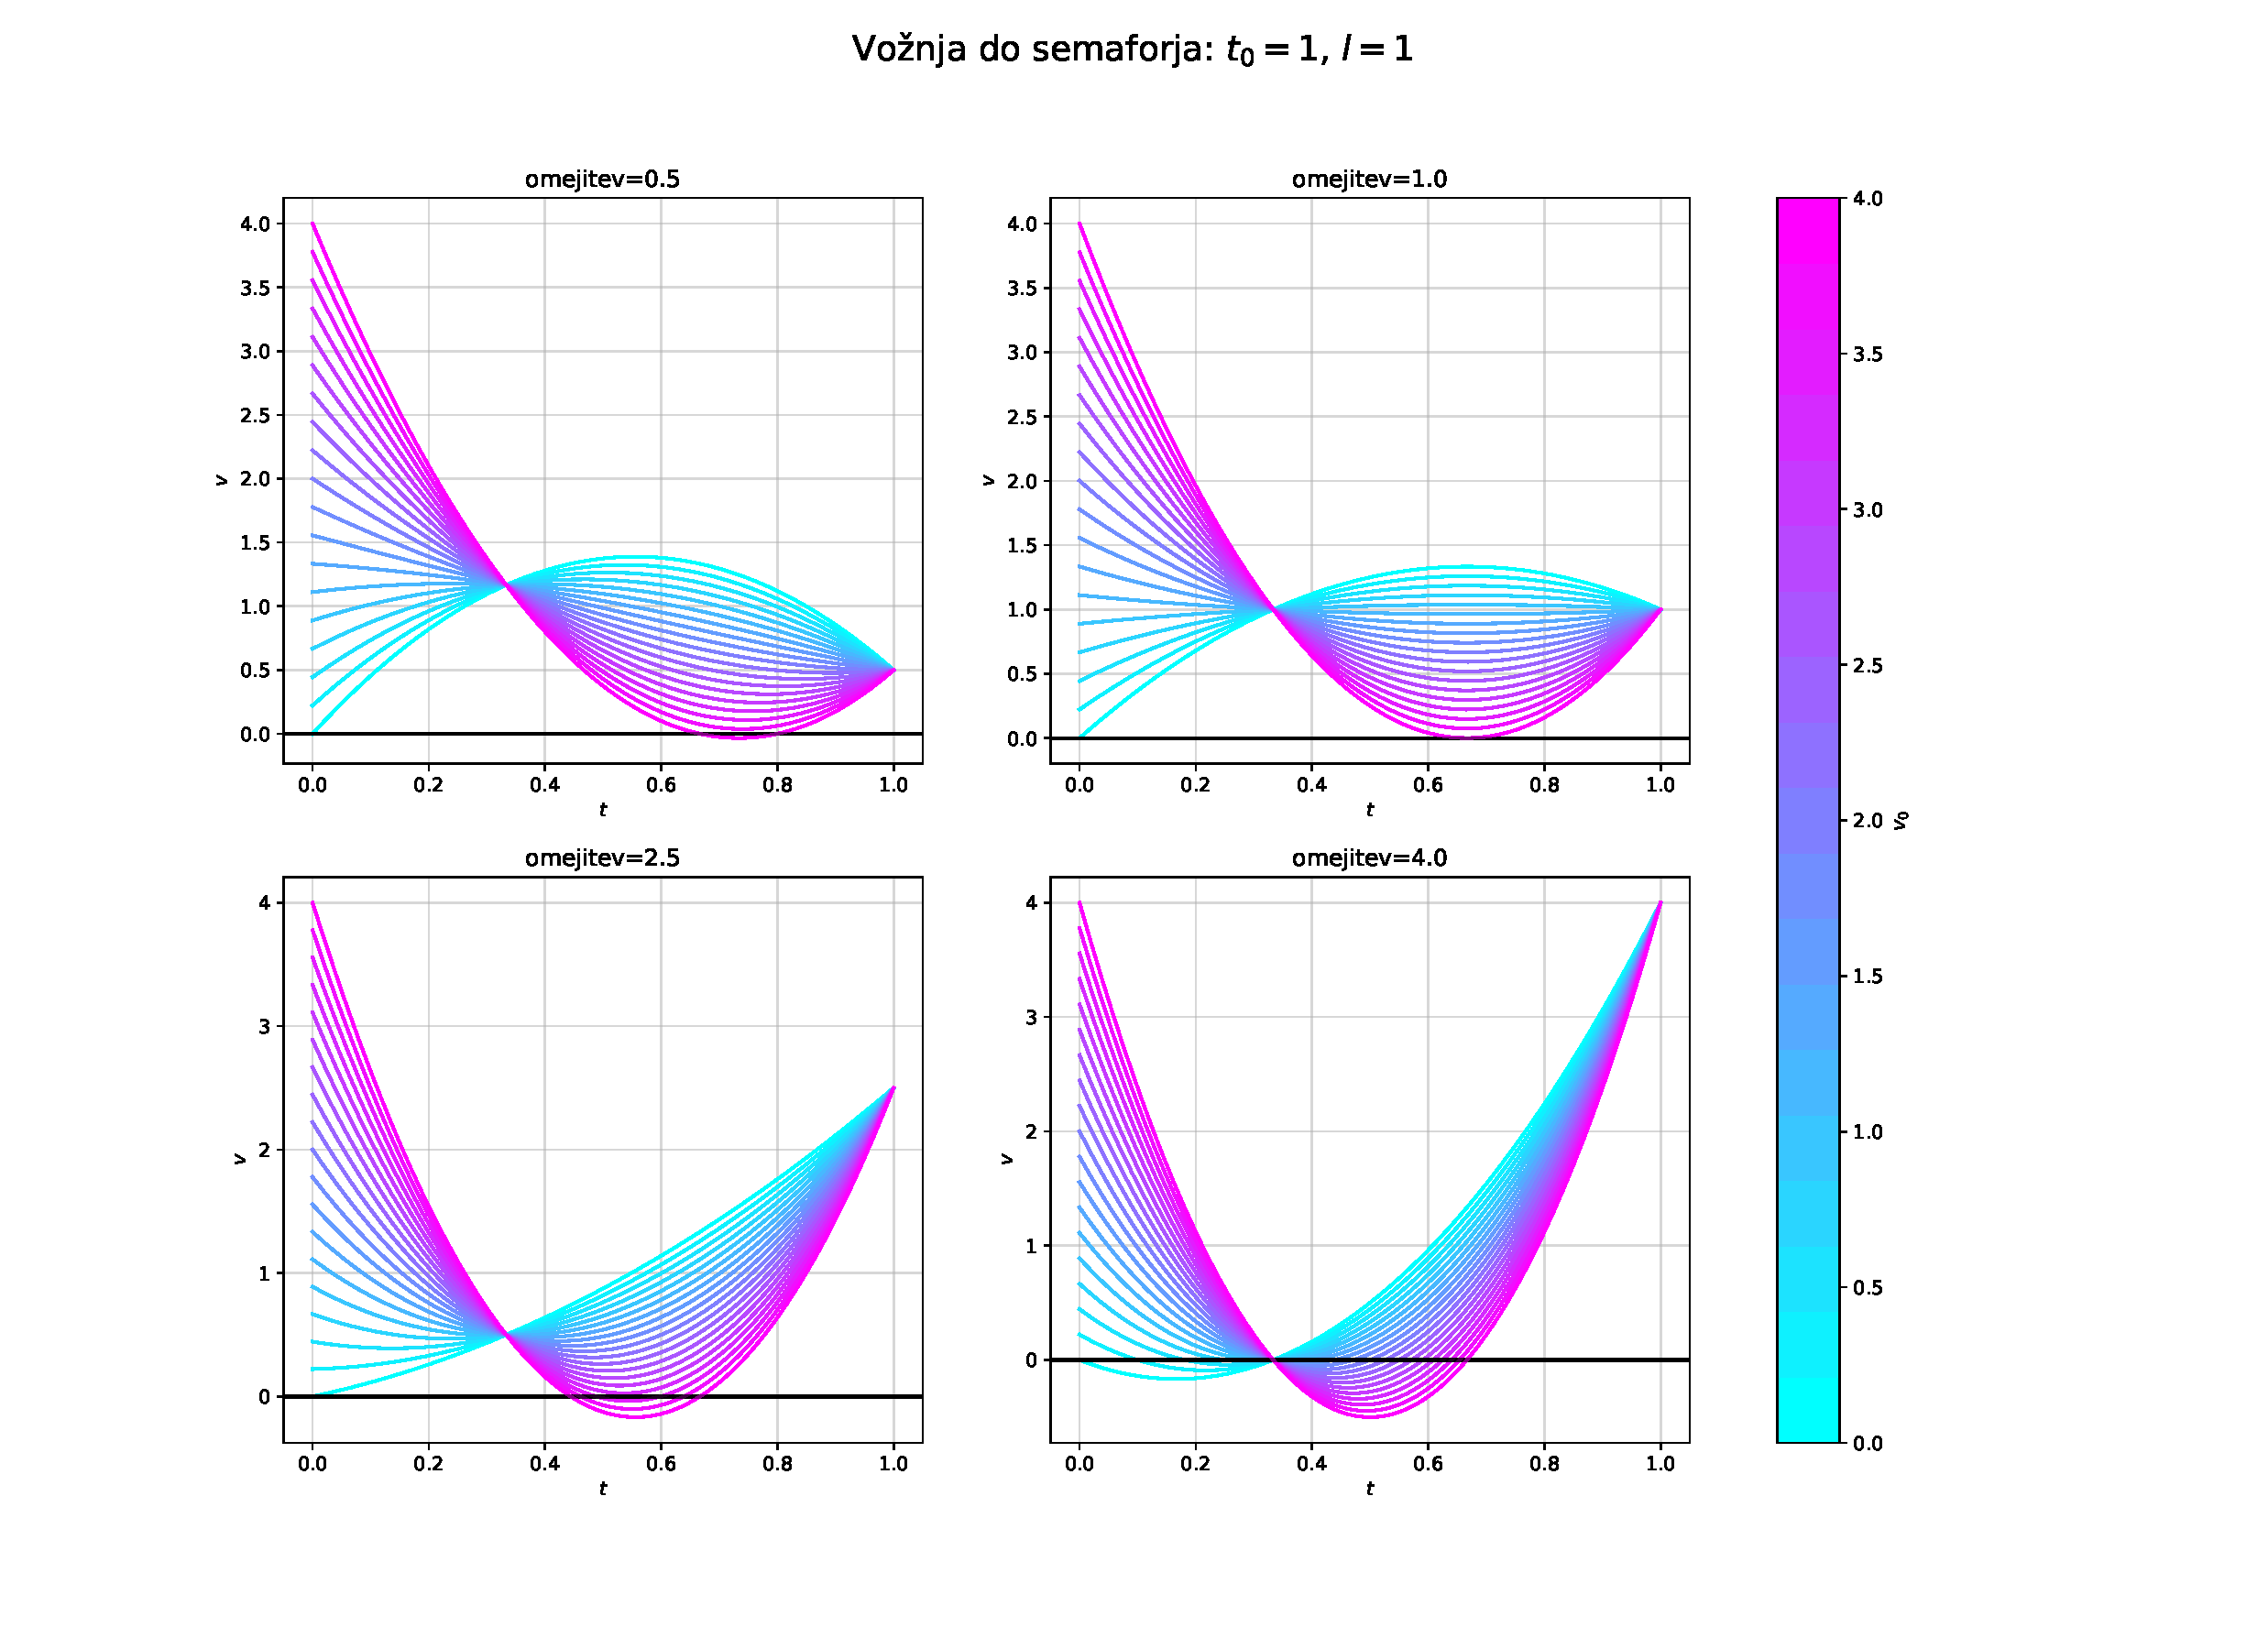
\includegraphics[width=0.95\textwidth]{grafi/dim_radar_1_1_omejitve.pdf}
\caption{Hitrosti v odvisnosti od časa za različne omejitve za semaforjem.}
\label{f:radar-omejitve}
\end{figure}




\section{Funkcional z višjimi potencami pospeška}
Pogoj za udobje vožnje spremenimo iz minimizacije kvadrata pospeška v minimizacijo višjih potenc. Lagrangian se prepiše v 
\begin{equation}
\lag = |\dot{v}|^p - \lambda v,
\end{equation}
funkcional v
\begin{equation}
F = \int_0^1 (|\dot{v}|^p - \lambda v)\diff t,
\end{equation}
E-L enačba pa 
\begin{equation}
p(p-1) |\dot{v}|^{p-2}\ddot{v} + \lambda = 0.
\label{e:lag-potence}
\end{equation}
Najprej si poglejmo primer, ko je potenca pospeška soda $p = 2n$, $n \in \mathbb{N}$. Enačbo \eqref{e:lag-potence} dvakrat integriramo in lahko izpustimo absolutne vrednosti. 
\begin{equation}
v(t) = - \frac{2n-1}{\lambda} \left( A - \frac{\lambda}{2n} t \right)^{\frac{2n}{2n-1}} + B
\end{equation}
Pri lihih potencah $p=2n+1$ integriramo \eqref{e:lag-potence} enkrat in dobimo
\begin{equation}
\frac{|\dot{v}|^p}{\dot{v}}=-\frac{\lambda}{p}t + A
\end{equation}
ter to enačbo prepišemo za lihe $p$  
\begin{equation}
\dot{v}^{2n}\frac{|\dot{v}|}{\dot{v}}=-\frac{\lambda}{2n+1}t + A
\end{equation}
Dobimo enako enačbo kot pri sodih potencah, le še dodatno funkcijo za predznak pospeška $\mathrm{sgn} \dot{v} = |\dot{v}|/\dot{v}$. Enačbo rešimo za oba primera, če je predznak pozitiven ali negativen. Za $\mathrm{sgn} \dot{v} = 1$ dobimo isto rešitev kot pri sodih potencah, za negativen predznak pa
\begin{equation}
v(t) = \frac{2n}{\lambda} \left(\frac{\lambda}{2n+1} t - A\right)^{\frac{2n+1}{2n}} + B
\end{equation}
Rešitev je tudi enaka primeru sodih potenc in lihih potenc s pozitivnim predznakom. Če zdaj prepišemo vse enačbe nazaj v obliko s $p$, dobimo za vse primere enačbo
\begin{equation}
v(t) = -\frac{p-1}{\lambda} \left(-\frac{\lambda}{p}t + A \right)^{\frac{p}{p-1}} + B.
\label{e:hitrost-p}
\end{equation}
Z upoštevanjem robnega pogoja na začetku, dolžine poti in odprtega robnega pogoja na koncu, dobimo šte vrednosti parametrov $A$, $B$ in $\lambda$. Enačba se prepiše v
\begin{equation}
v_p(t) = \frac{2p-1}{p}(1-v_0)\left( 1-(1-t)^{\frac{p}{p-1}} \right) + v_0.
\end{equation}
\begin{figure}[H]
\centering
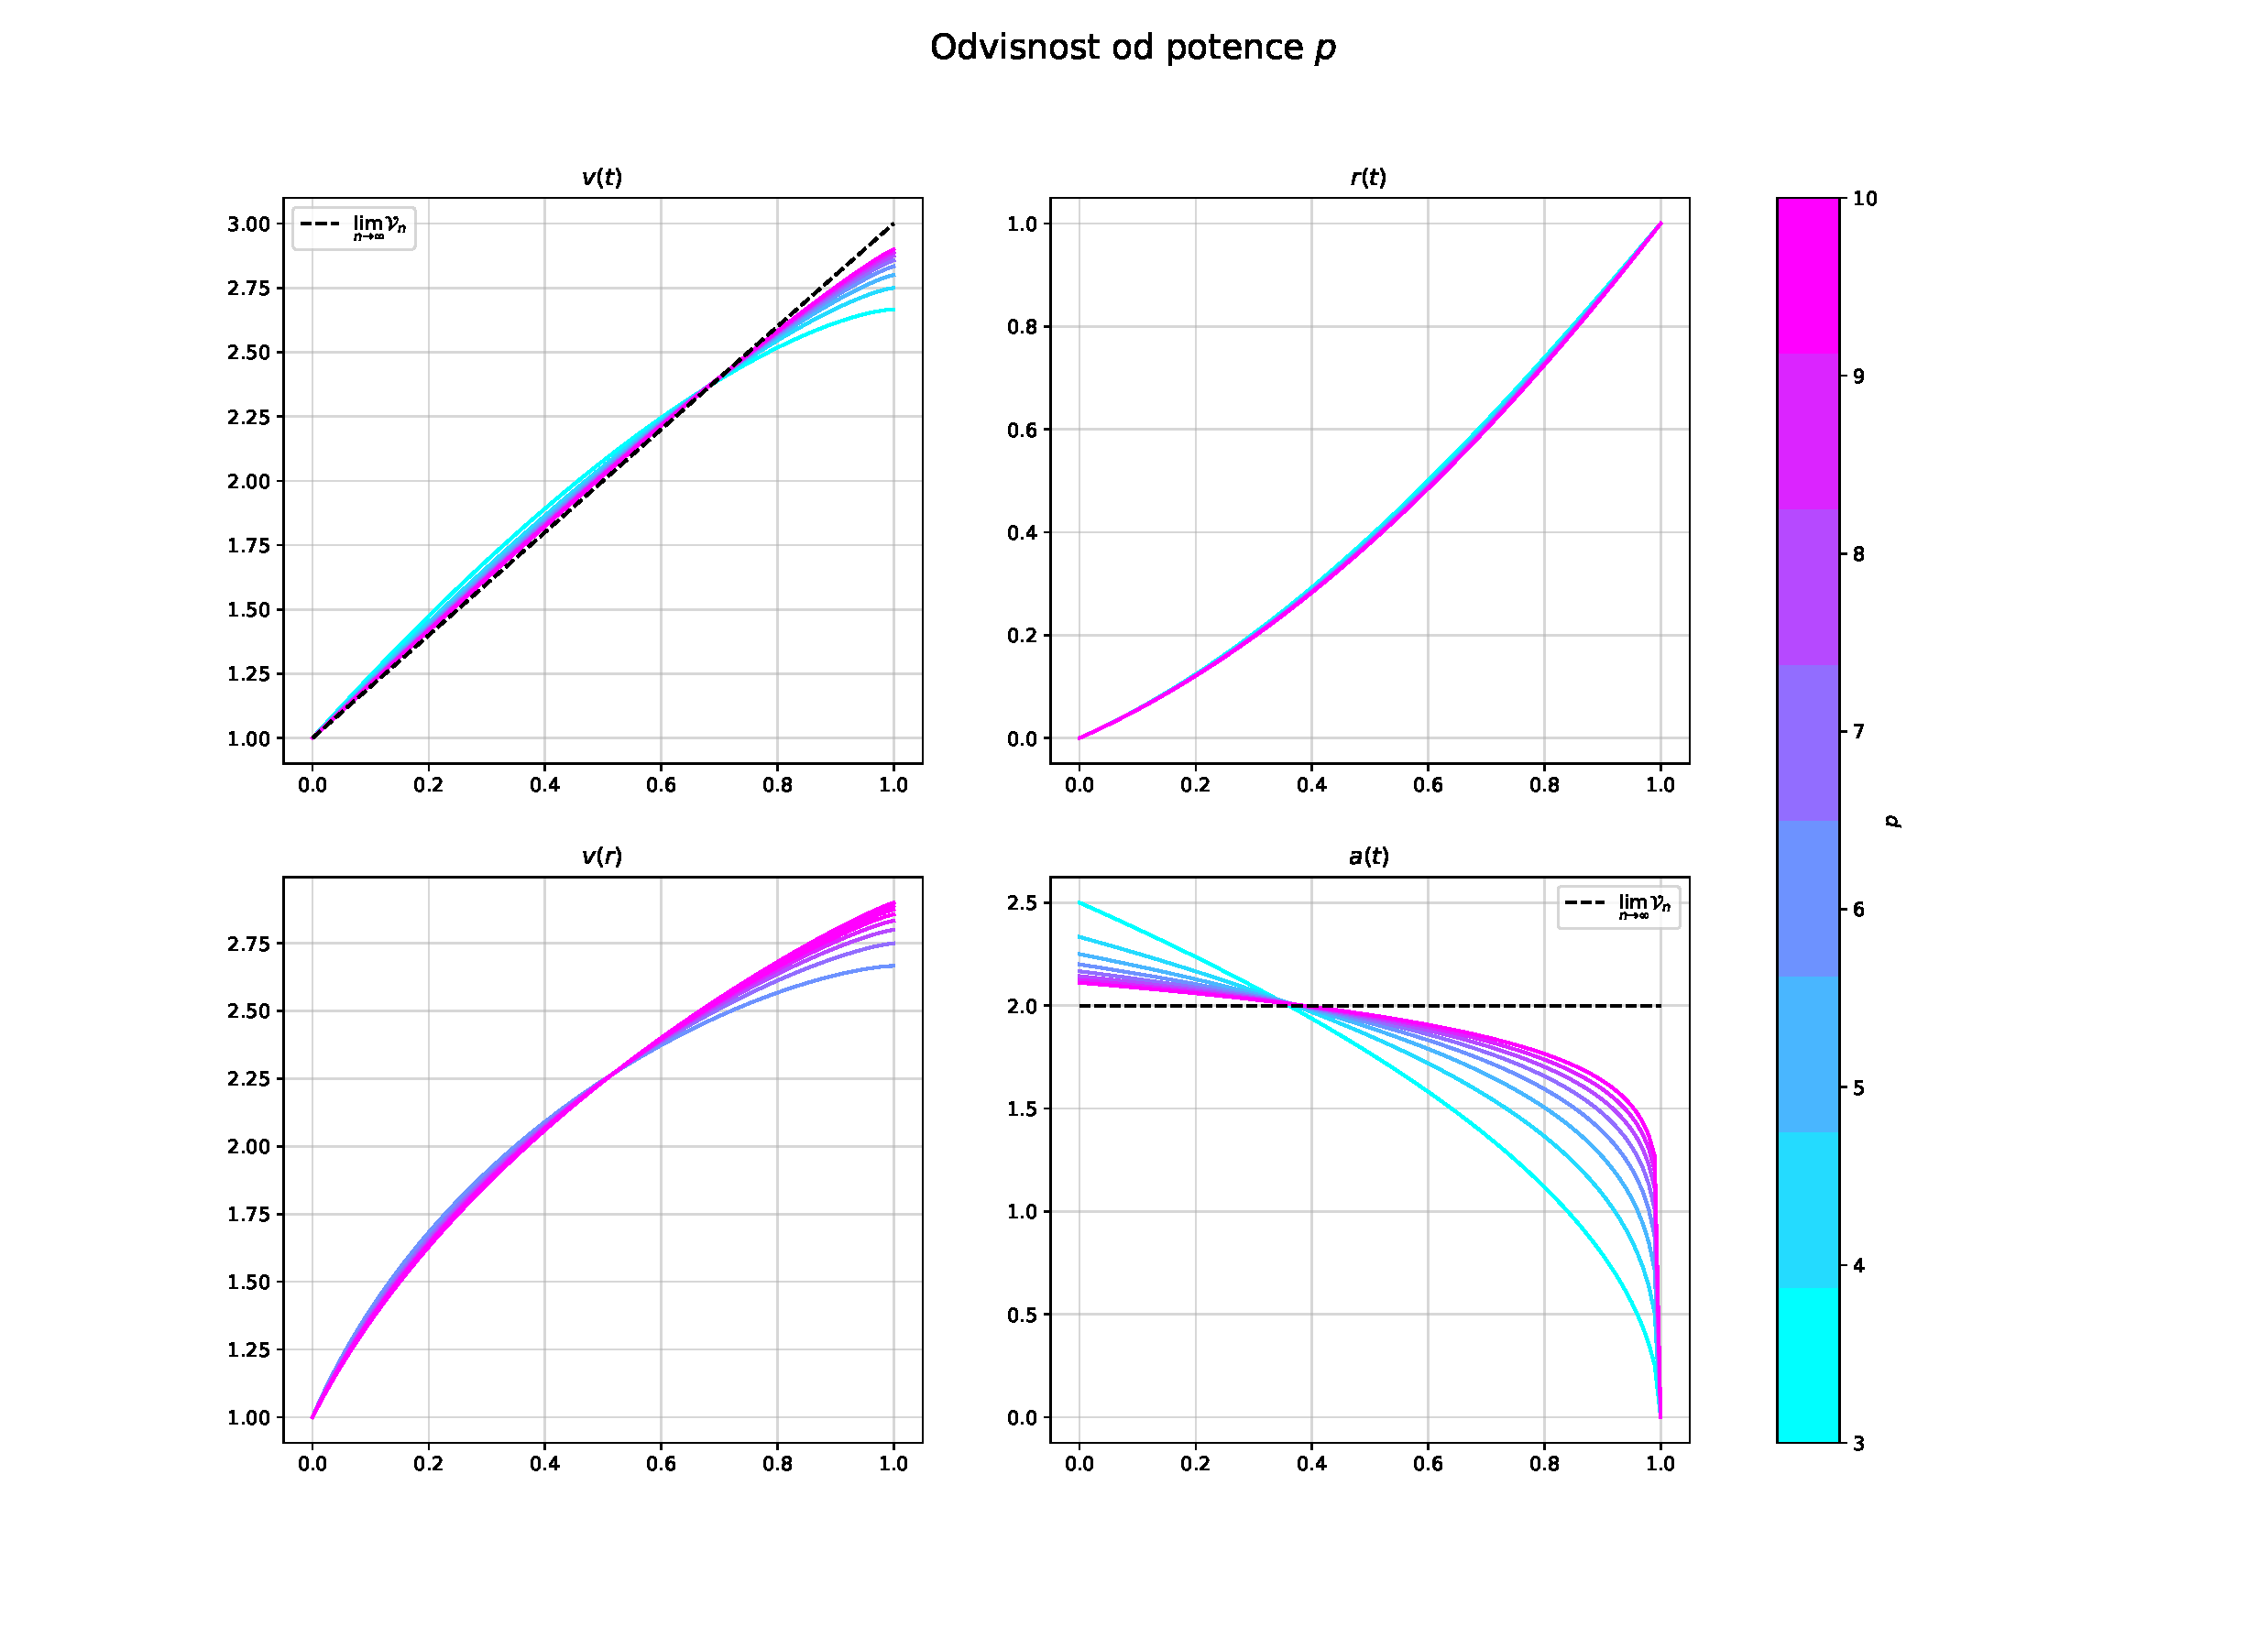
\includegraphics[width=0.95\textwidth]{grafi/odvisnost_p_ult.pdf}
\caption{Hitrosti v odvisnosti od potence $p$ pospeška v funkcionalu.}
\label{f:p}
\end{figure}
Poglejmo si še dogajanje v limiti $p \rightarrow \infty$. Iz grafov hitrosti za različne $p$ (slika \ref{f:p}) nam je takoj jasno, da se bo hitrost spreminjala linearno, to pa podpira tudi enačba
\begin{equation}
v_{\infty}(t) =  2(1-v_0)t + v_0.
\end{equation}




\section{Dodatni člen $v^2$}
V tem delu naloge pa spremenimo Lagrangian tako, da vključimo še člen s kvadratom hitrosti, da ostanemo pri cesti primernih hitrostih.
\begin{equation}
\lag = \dot{v}^2 + \mu v - \lambda v
\end{equation}
Parameter $\mu$ je nekakšen faktor pomembnosti člena s kvadratom hitrosti. Določili ga bomo z numeričnimi poskusi. V tem primeru se funkcional glasi
\begin{equation}
F = \int_0^1(\dot{v}^2 + \mu v^2 - \lambda v)\diff t,
\end{equation}
E-L enačba pa nam da
\begin{equation}
\ddot{v} - \mu v + \frac{\lambda}{2} = 0
\end{equation}
Rešitev te diferencialne enačbe je
\begin{equation}
v(t) = \frac{\lambda}{2\mu} + Ae^{\sqrt{\mu}t} + Be^{-\sqrt{\mu}t}
\end{equation}
Ob upoštevanju robnih pogojev za ekstremno hitrost pri semaforju in vez \eqref{e:vez}, dobimo rešitev za hitrost
\begin{equation}
v(t) = \frac{\lambda}{2\mu} + \frac{v_0 - \frac{\lambda}{2\mu}}{1 + e^{2\sqrt{\mu}}} \left( e^{t\sqrt{\mu}} + e^{-\sqrt{\mu}(2-t)} \right)
\end{equation}
Reševanje enačbe bom nadaljeval numerično, da se izodnem dolgem računanju $\lambda$. Za različne faktorje $\mu$ sem izračunal potek gibanja in ga prikazal na sliki \ref{f:hitrost-funkc}. \par\vspace{5mm}

Po pričakovanjiih se z večanjem $\mu$ hitrost gibanja manjša, saj člen s hitrostjo postaja vedno pomembnejši od člena s pospeškom. Tako lahko nekoliko omejimo hitrost, vendar neželen stranski efekt je neudobna vožnja. Pospešek pri velikih $\mu$ postane velik na začetku, v nadaljevanju vožnje pa pade na 0. Iz grafa lahko razberemo, da je pametna izbira za ta parameter nekje na intervalu $\mu \in [5, 10]$. Pri manjših vrednostih na hitrost skoraj ne vplivamo, pri višjih pa vožnja ni več udobna.

\begin{figure}[H]
\centering
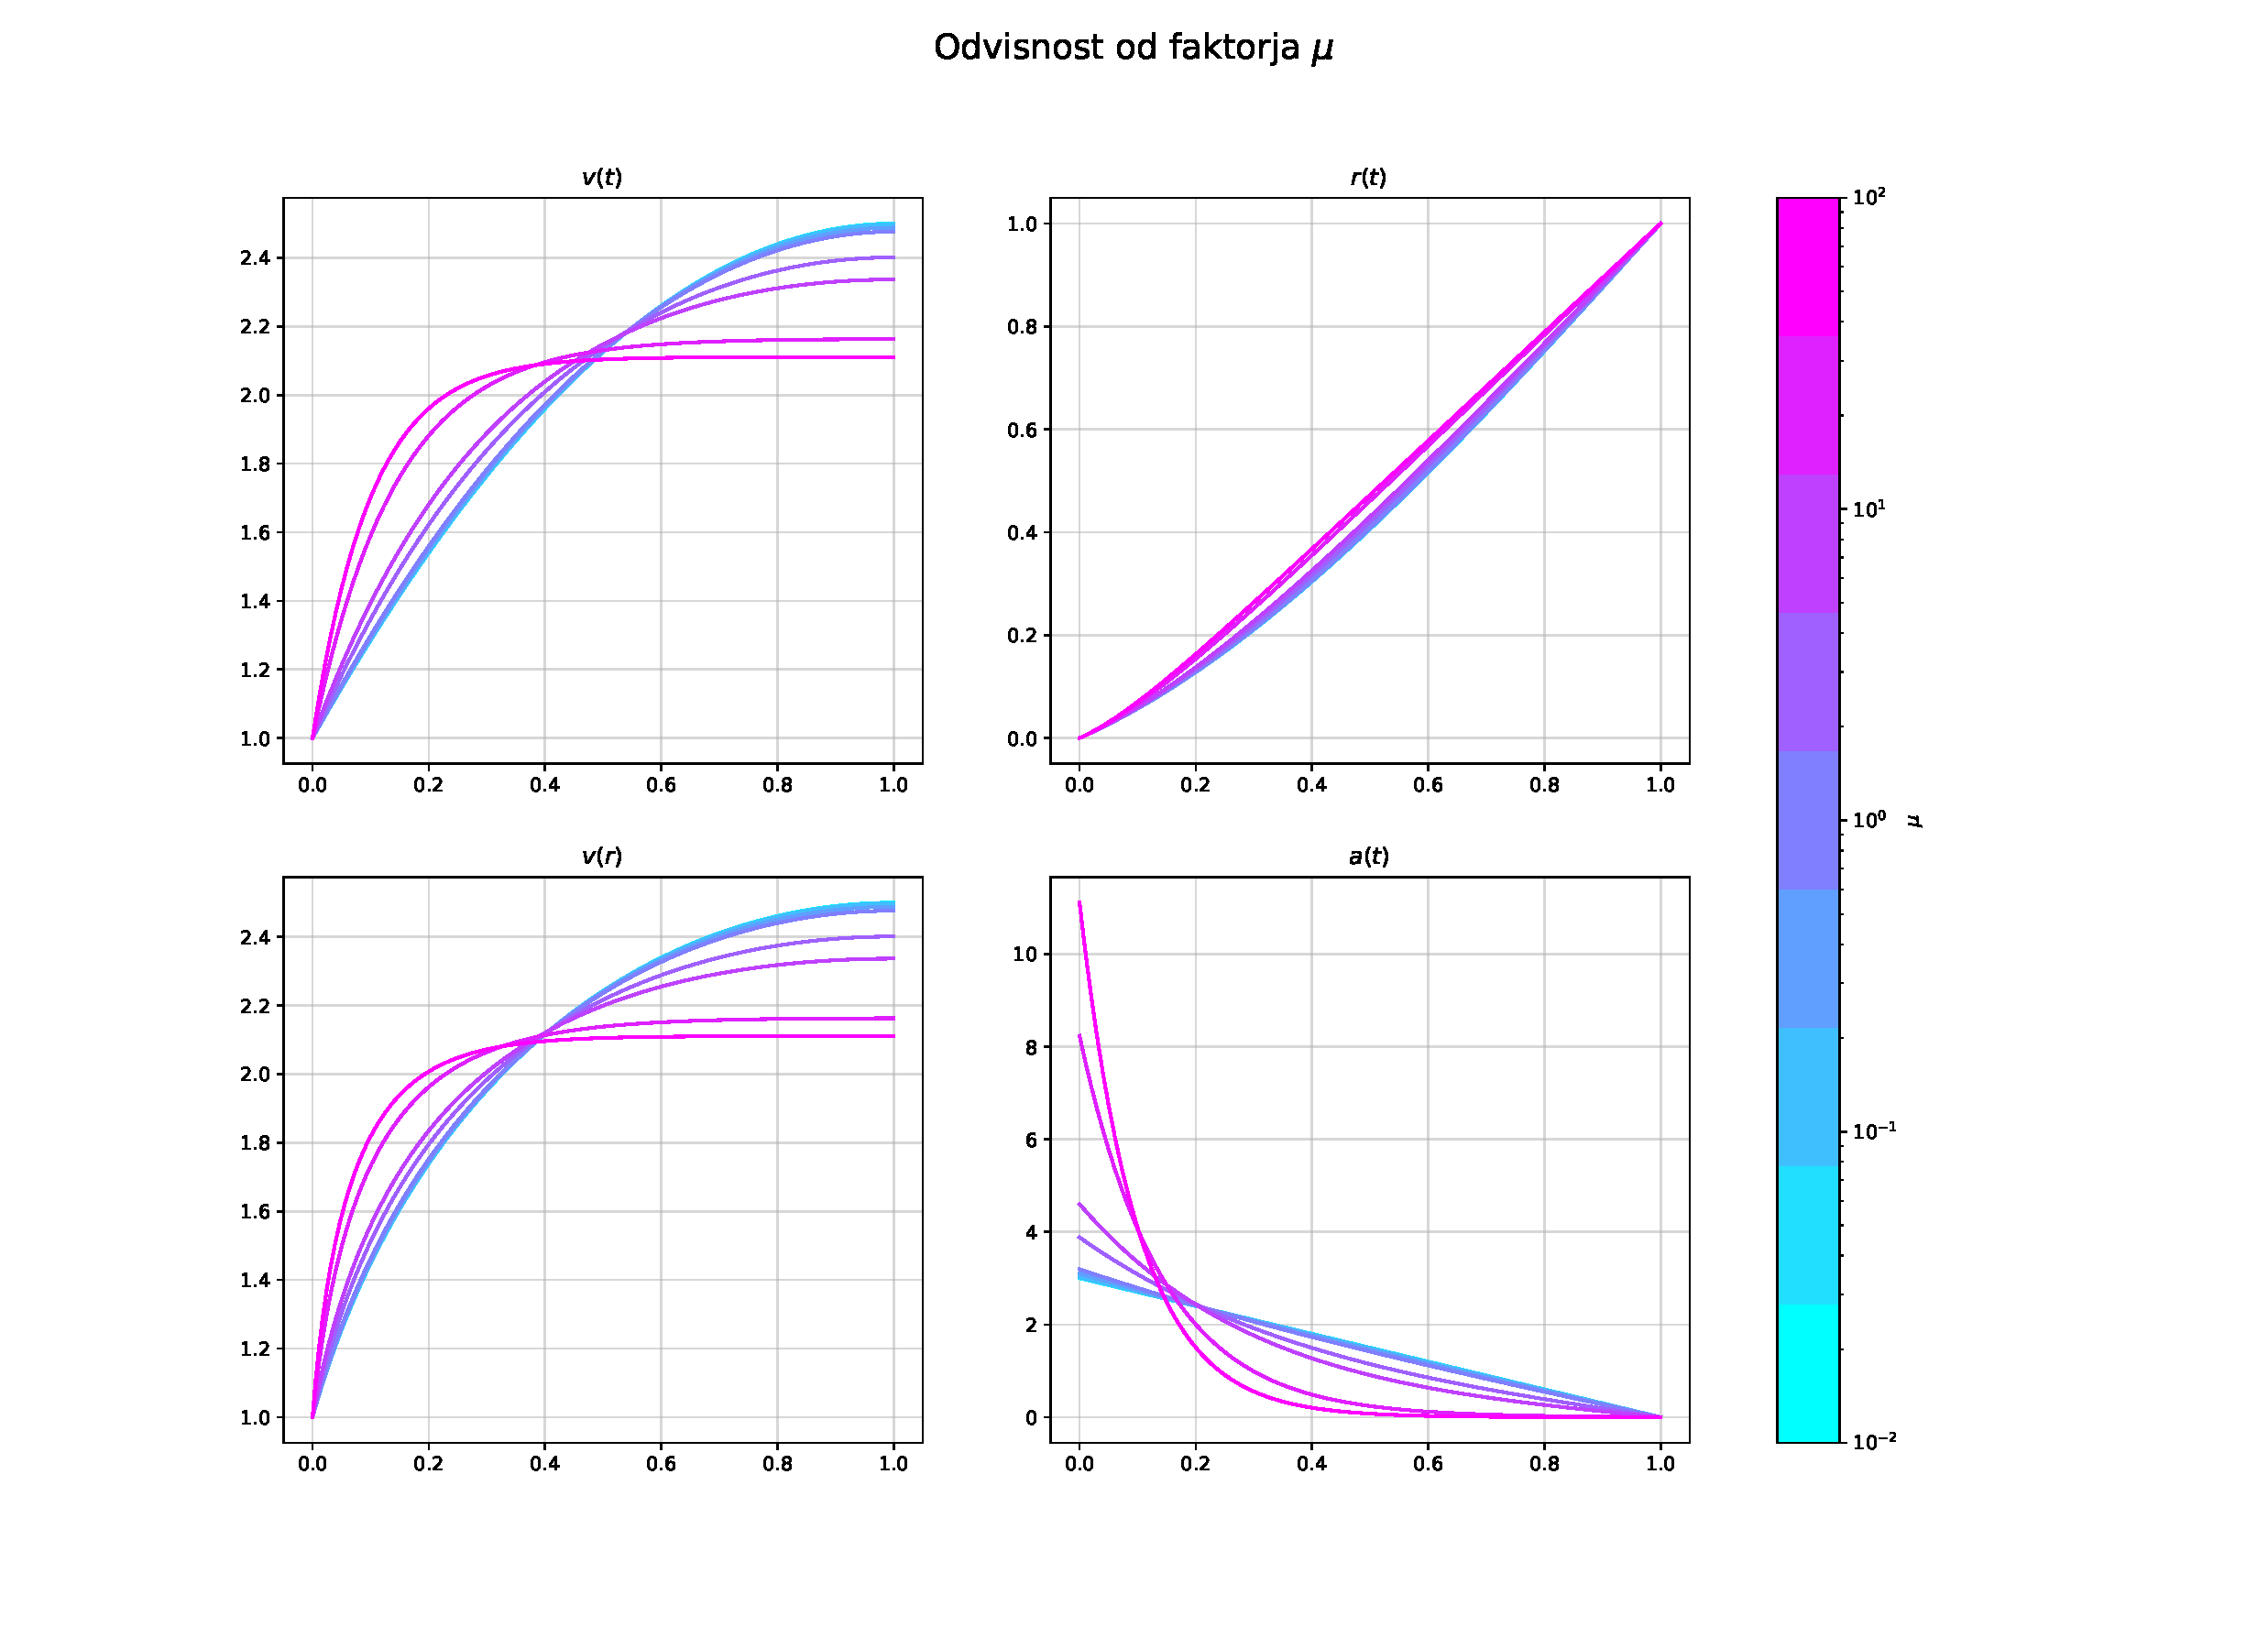
\includegraphics[width=0.95\textwidth]{grafi/hitrostni_potencial.pdf}
\caption{Gibanje za Lagrangian z dodatnim členom $v^2$ za različne faktorje $\mu$.}
\label{f:hitrost-funkc}
\end{figure}



\section{Zaporedni semaforji}
Za konec si poglejmo še problem $n$ zaporednih semaforjev na enakomernih razmakih $l$. V taki situaciji se v Sloveniji težko znajdemo, je pa veliko bolj pogosta v večjih ameriških mestih s ponavljajočo strukturo. \par\vspace{5mm}

\begin{figure}[H]
\centering
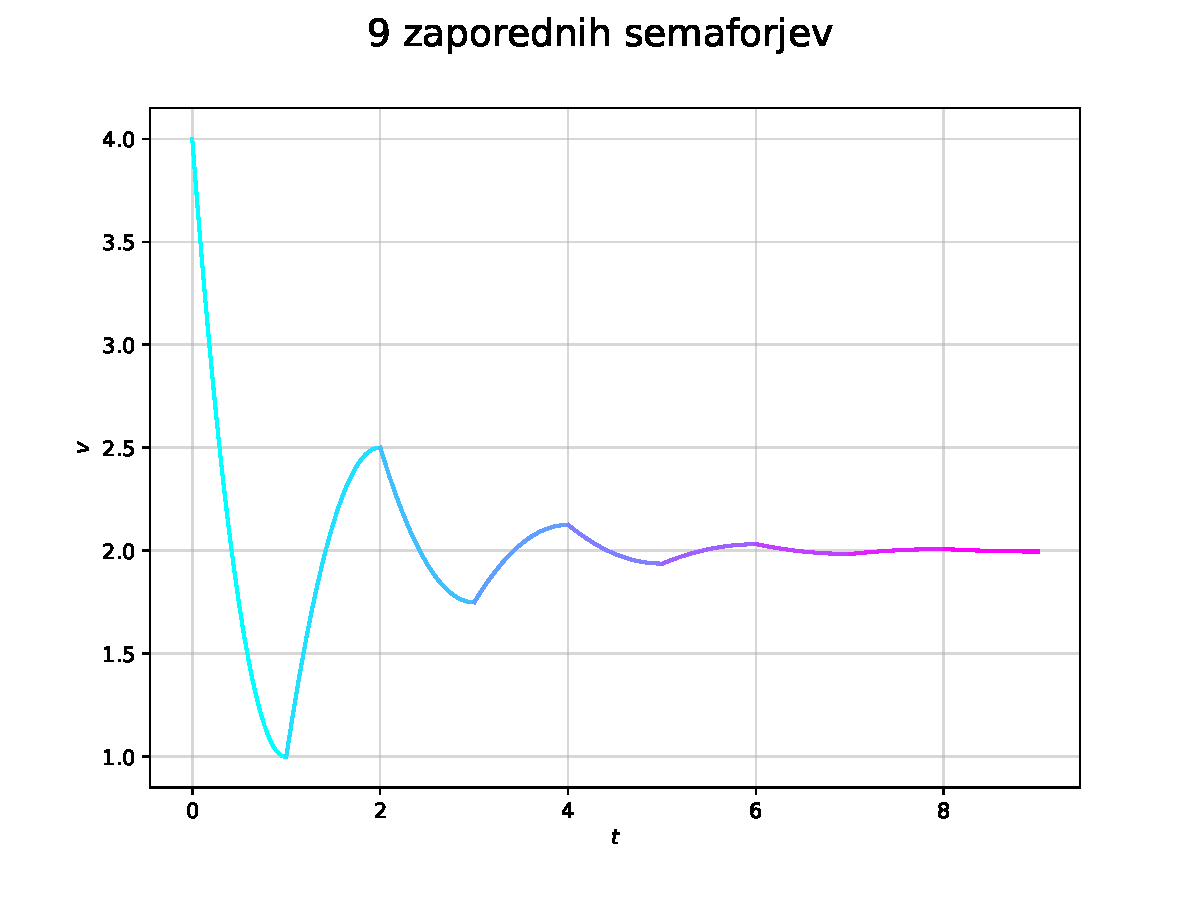
\includegraphics[width=0.50\textwidth]{grafi/zaporedni_9.pdf}
\caption{Hitrost skozi 9 zaporednih semaforjev.}
\label{f:zaporedni-bad}
\end{figure}

Reševanja tega problema se bom lotil numerično s pomočjo knjižnice \texttt{scipy.integrate. solve_bvp} v programskem jeziku \texttt{Python}. Obravnaval ga bom kot setijo problemov iz prvega poglavja, dodatno pa velja, da je končna hitrost enega problema začetna hitrost naslednjega
\begin{equation}
v_1(0) = v_0, \qquad v_{i+1}(0) = v_i(1).
\end{equation}
Rezultat je prikazan na sliki \ref{f:zaporedni-bad}. Vidimo, da hitrost ni zvezna, ampak pospeški se po vsakem semaforju manjši in hitrost konvergira proti povprečni. \par\vspace{5mm}

Taka vožnja ni ravno udobna, zato zahtevamo še zveznost odvoda hitrosti. Kot prej imamo v $i$-tem odseku prabolo
\begin{equation}
v(t) = a_it^2 + b_it + c_i
\end{equation}
in robnimi pogoji
\begin{eqnarray}
v_i(0) = v_0, \qquad v_{i+1}(0) = v_i(1) \\
\dot{v}_{i+1}(0) = \dot{v}_i(1)
\end{eqnarray}
Dobimo serijo zlepljenih parabol (slika \ref{f:zaporedni}). Uspešno smo zgladili hitrost. Problem te metode je, da divergira pri kasnejših semaforjih.

\begin{figure}[H]
\centering
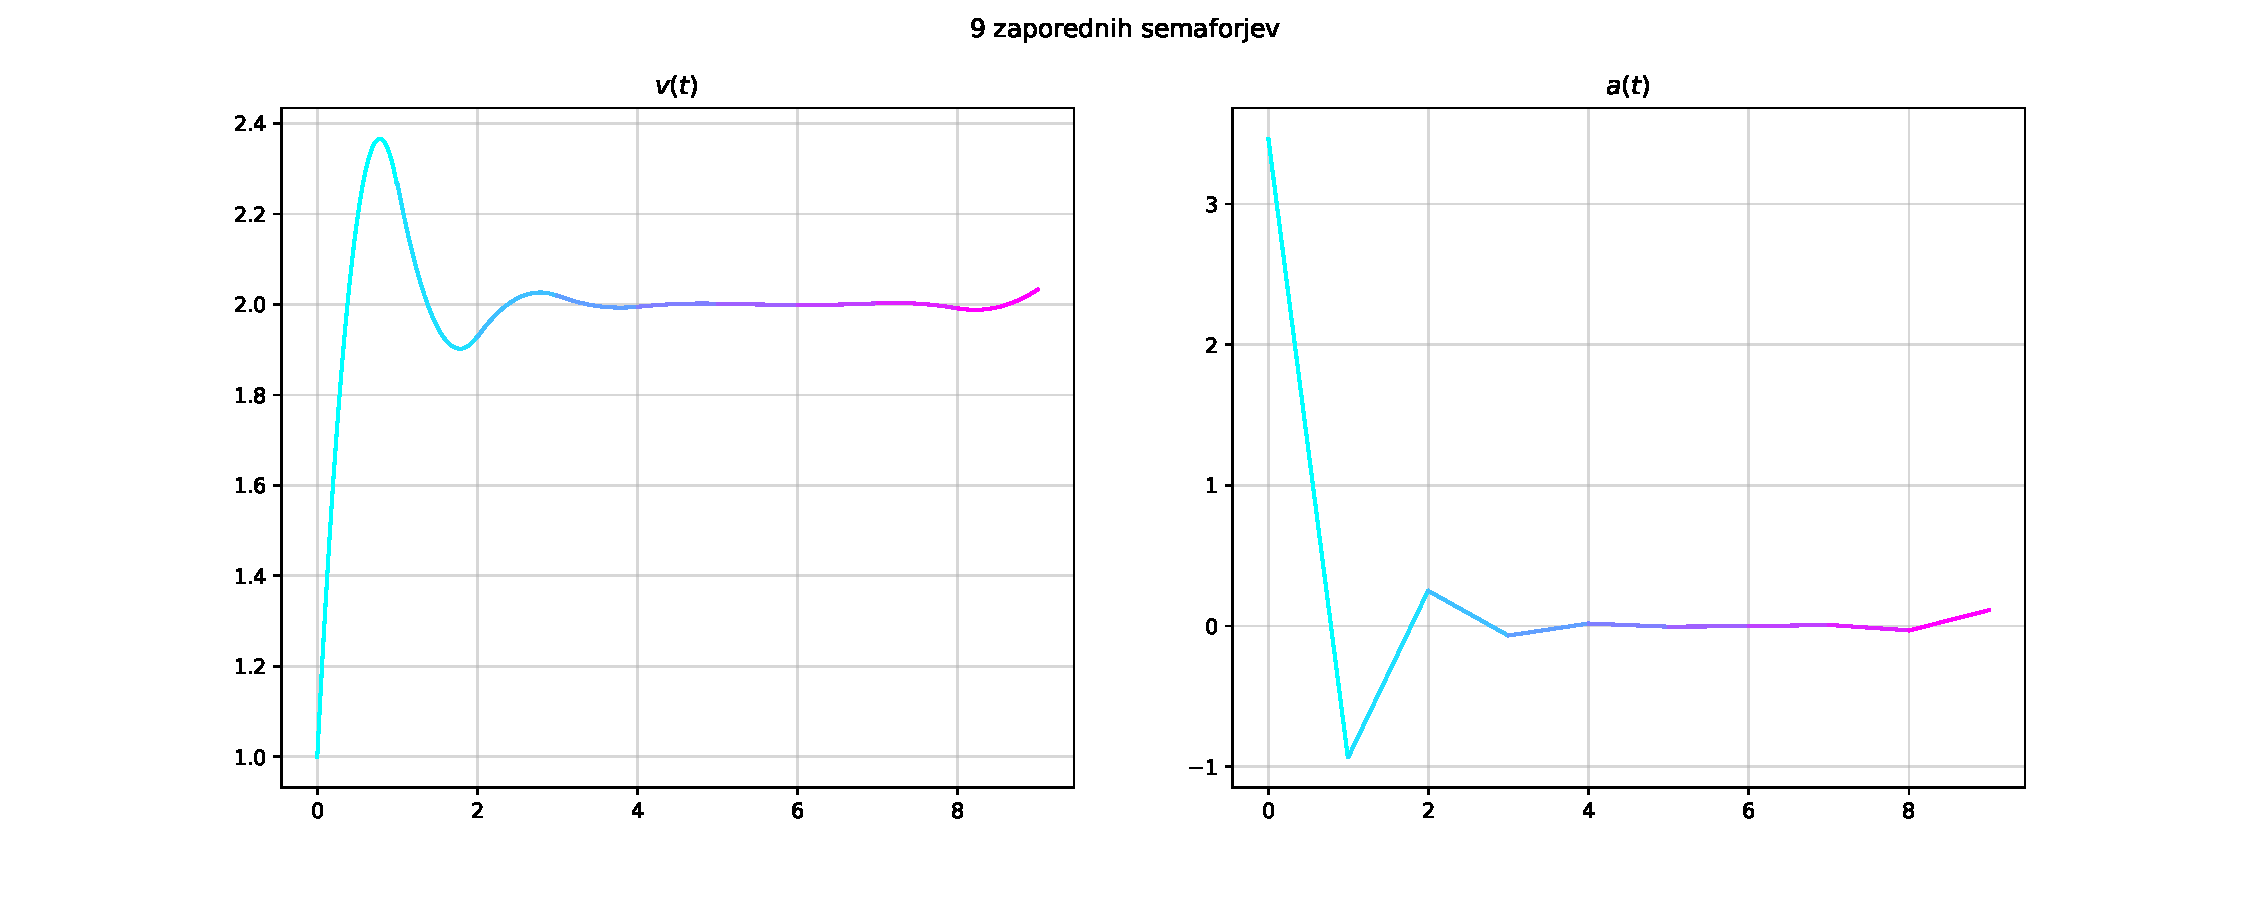
\includegraphics[width=0.95\textwidth]{grafi/zaporedni_fin_9.pdf}
\caption{Hitrost in pospešek pri gibanju skozi 9 zaporednih semaforjev.}
\label{f:zaporedni}
\end{figure}



\end{document}